\section{Blind ATLAS data sample testing}\label{sec:blind_test}
The final test to run on the autoencoder is a blind test. The blind test will compare the
reconstruction error from the autoencoder on an ATLAS dataset with the reconstruction error
on the same ATLAS dataset where about 1.6 million events have been randomly removed and 
switched with samples from many BSM samples. The signal samples have been given the same 
weight as the ATLAS data. Therefor the total amount of events before eventselection are the same
in both datasets. The dataset was prepared by one of the supervisors of this thesis, and not shown 
to the author. The ATLAS data contains events from the data collection from 2015 and 2016, and 
the signal samples are created according to those runs. The ATLAS data will therefor be referred to 
as ATLAS data 15 and data 16 for the ATLAS events, and the mix set will be referred to data1516 mix. 


\begin{figure}[!htb]
\centering
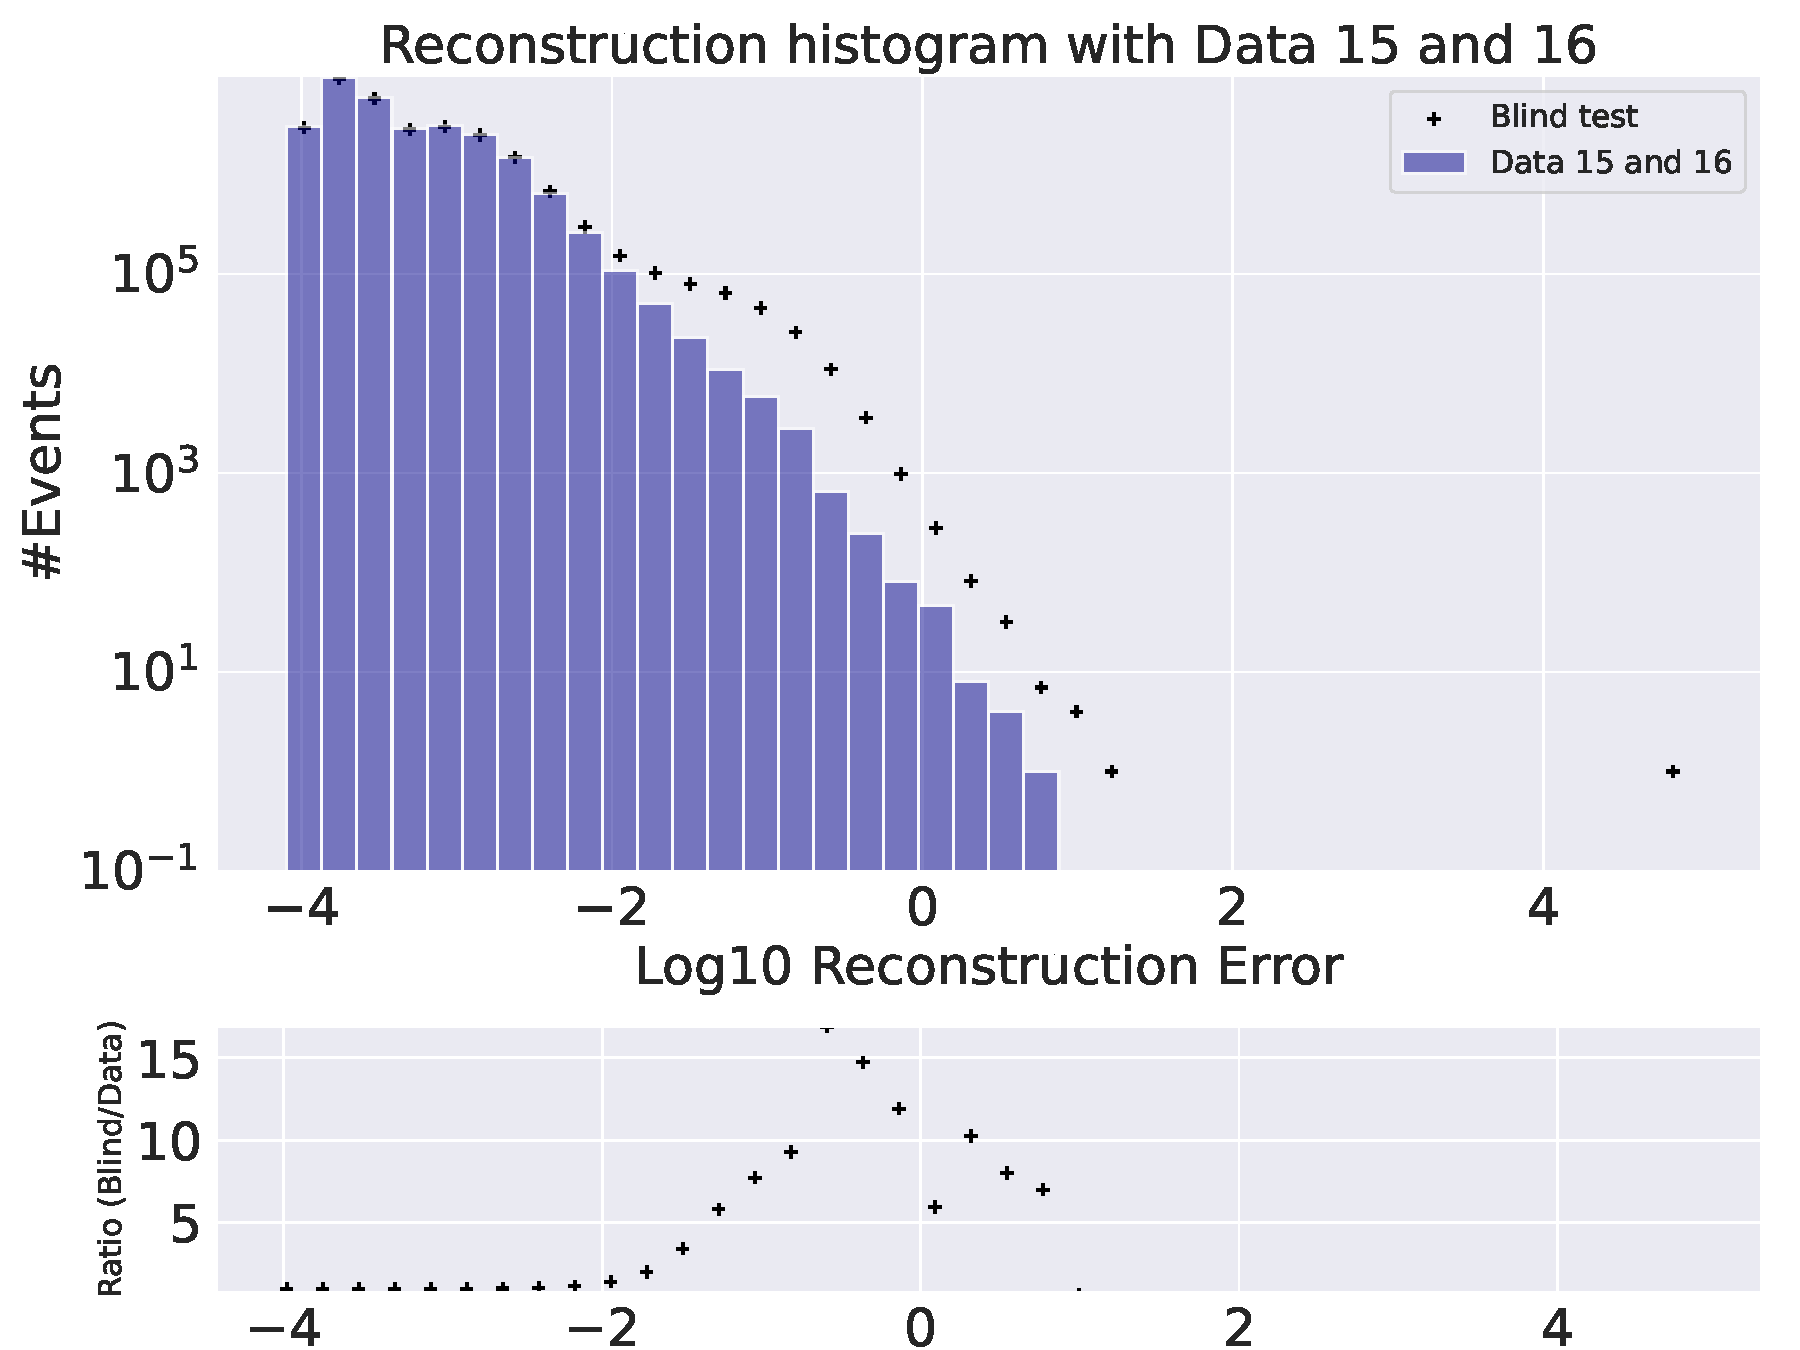
\includegraphics[width=\linewidth]{Figures/AE_testing/blindtest/b_data_recon_big_rm3_feats_sig_Blind test_.pdf}
\caption[Reconstruction error blind test]{Reconstruction error for the blind test. The 
blue histogram is the ATLAS data 15 and data 16 sample and the black crosses are the 
 ATLAS data mixed with BSM samples. Between a reconstruction error of $10^{-2}$ and $10^{0.5}$
 there is a separation of the peaks of the two distributions. The biggest difference is a ratio difference of around 15.}
\label{fig:blind_test_reconerr}
\end{figure}

In figure \ref{fig:blind_test_reconerr} the reconstruction error for the blind test is shown.
The ratio subplot beneath the histogram shows the reconstruction error discrepancy. 
This indicates that the autoencoder is able to distinguish between the ATLAS data 15 and data 16, and BSM samples. 
The highest ratio difference is around 15 between the two datasets. The ratio discrepancy is also 
due to event selection. The mix set contains the same events as the ATLAS data 15 and data 16 sample set, but has 
around 1.6 million ATLAS events removed and replaced with BSM events. It appears that a higher number 
of BSM signal samples than the events that was removed passed the cuts in event selection. \par
The model has not been changed after running inference on the blind test, and we can therefor unblind the 
test, and see how well the autoencoder actually did in separating out the BSM events. 

\begin{figure}[!htb]
    \centering
    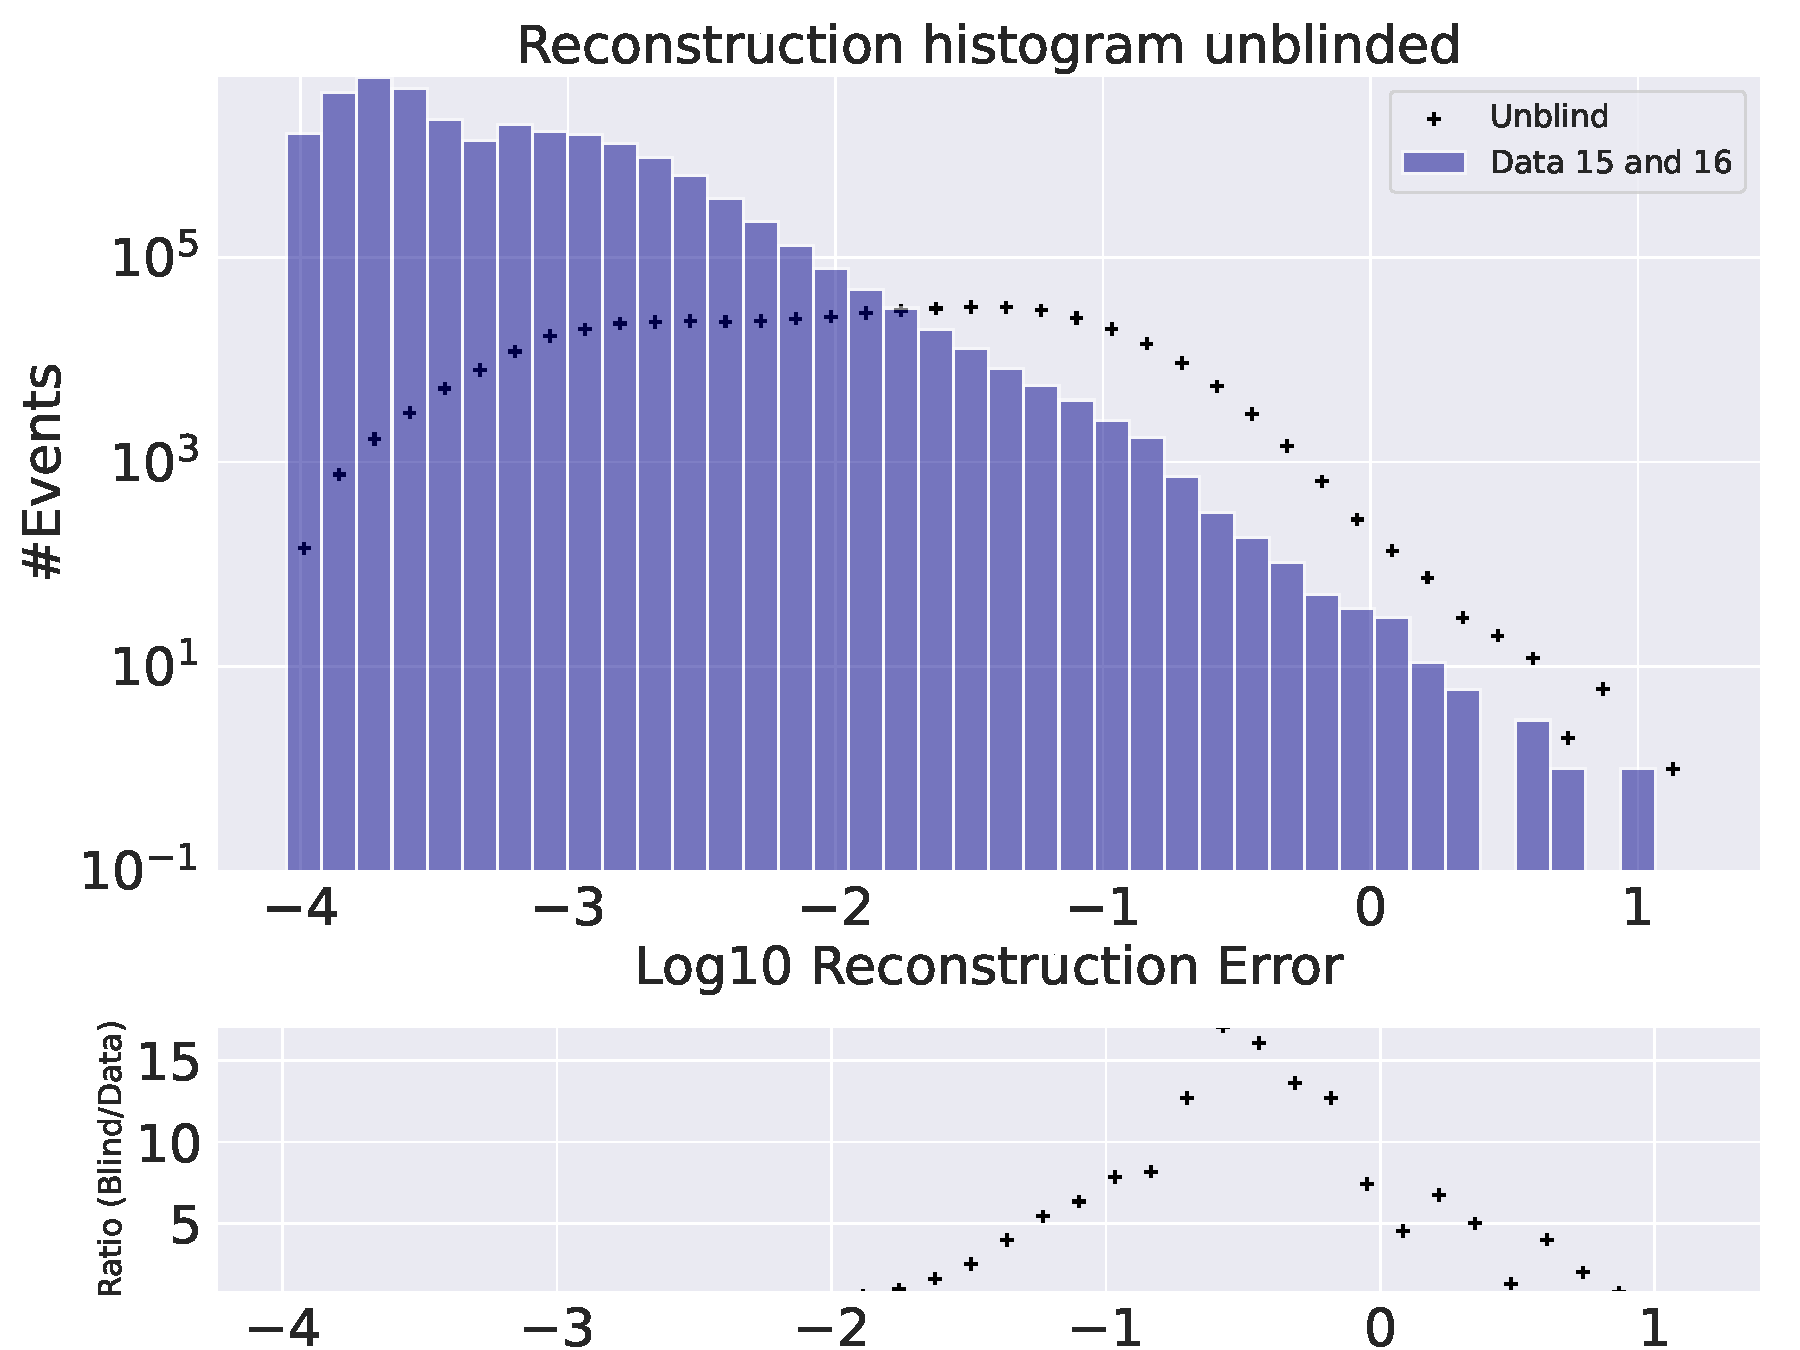
\includegraphics[width=\linewidth]{Figures/AE_testing/blindtest/b_data_recon_big_rm3_feats_sig_Unblind_.pdf}
    \caption[Reconstruction error unblind test]{Reconstruction error for the unblind test. In the histogram the 
    blue bins are the ATLAS data 15 and data 16 samples from the mix dataset and the black crosses are the 
    BSM samples with the legend "Unblind". Between a reconstruction error of $10^{-2}$ and $10^{0.5}$
     there is a separation of peaks of the two distributions. The biggest difference is a ratio 
     difference of around 15.}
    \label{fig:unblind_test_reconerr}
\end{figure}

In figure \ref{fig:unblind_test_reconerr} the reconstruction error distributions for both ATLAS data 15 and data 16 samples, 
and BSM signals samples are shown. Allthough some samples have low reconstruction error, the peak is
between $10^{-2}$ and $10^{0.5}$ reconstruction error. The hishget ratio discrepancy is around 15 between the two distributions,
and it is shown to be in the same area of the peak. 